%%%%%%%%%%%%%%%%%%%%%%%%%%%%% Define Article %%%%%%%%%%%%%%%%%%%%%%%%%%%%%%%%%%
\documentclass{report}
%%%%%%%%%%%%%%%%%%%%%%%%%%%%%%%%%%%%%%%%%%%%%%%%%%%%%%%%%%%%%%%%%%%%%%%%%%%%%%%

%%%%%%%%%%%%%%%%%%%%%%%%%%%%% Using Packages %%%%%%%%%%%%%%%%%%%%%%%%%%%%%%%%%%

\usepackage[utf8]{inputenc}
% \usepackage{float}
% \usepackage{geometry}
% \usepackage{amssymb}
% \usepackage{amsthm}
% \usepackage{amsmath}
\usepackage{graphicx}
\graphicspath{{images/}}
\usepackage[breaklinks]{hyperref}
\usepackage{listings}
% \usepackage{pdfpages}
% \usepackage{comment}
% \usepackage{fancyhdr}
% \usepackage[english]{babel}
% \usepackage{empheq}
% \usepackage{mdframed}
% \usepackage{booktabs}
% \usepackage{lipsum}
% \usepackage{color}
% \usepackage{psfrag}
% \usepackage{pgfplots}
% \usepackage{bm}
% \usepackage{wrapfig}
% \usepackage{bookmark}
% \usepackage{titlesec}
\usepackage{hyperref}
%%%%%%%%%%%%%%%%%%%%%%%%%%%%%%%%%%%%%%%%%%%%%%%%%%%%%%%%%%%%%%%%%%%%%%%%%%%%%%%

% Other Settings
\hypersetup{
    colorlinks = true,
    linkcolor = black,
    urlcolor = blue,
}
\urlstyle{same}

% \titleformat{\chapter}[display]
%   {\normalfont\bfseries}{}{0pt}{\Huge}

% %%%%%%%%%%%%%%%%%%%%%%%%%% Page Setting %%%%%%%%%%%%%%%%%%%%%%%%%%%%%%%%%%%%%%%
% \geometry{a4paper}
% \pagestyle{fancy}
% \fancyhead{}
% \fancyhead[L]{Project Report}
% \fancyhead[C]{RISC-V Processor}
% \fancyhead[R]{Computer Architecture}
% \fancyfoot{}
% \fancyfoot[C]{\thepage}

% %%%%%%%%%%%%%%%%%%%%%%%%%% Define some useful colors %%%%%%%%%%%%%%%%%%%%%%%%%%
% \definecolor{ocre}{RGB}{243,102,25}
% \definecolor{mygray}{RGB}{243,243,244}
% \definecolor{deepGreen}{RGB}{26,111,0}
% \definecolor{shallowGreen}{RGB}{235,255,255}
% \definecolor{deepBlue}{RGB}{61,124,222}
% \definecolor{shallowBlue}{RGB}{235,249,255}
% %%%%%%%%%%%%%%%%%%%%%%%%%%%%%%%%%%%%%%%%%%%%%%%%%%%%%%%%%%%%%%%%%%%%%%%%%%%%%%%

% %%%%%%%%%%%%%%%%%%%%%%%%%% Define an orangebox command %%%%%%%%%%%%%%%%%%%%%%%%
% \newcommand\orangebox[1]{\fcolorbox{ocre}{mygray}{\hspace{1em}#1\hspace{1em}}}
% %%%%%%%%%%%%%%%%%%%%%%%%%%%%%%%%%%%%%%%%%%%%%%%%%%%%%%%%%%%%%%%%%%%%%%%%%%%%%%%

% %%%%%%%%%%%%%%%%%%%%%%%%%%%% English Environments %%%%%%%%%%%%%%%%%%%%%%%%%%%%%
% \newtheoremstyle{mytheoremstyle}{3pt}{3pt}{\normalfont}{0cm}{\rmfamily\bfseries}{}{1em}{{\color{black}\thmname{#1}~\thmnumber{#2}}\thmnote{\,--\,#3}}
% \newtheoremstyle{myproblemstyle}{3pt}{3pt}{\normalfont}{0cm}{\rmfamily\bfseries}{}{1em}{{\color{black}\thmname{#1}~\thmnumber{#2}}\thmnote{\,--\,#3}}
% \theoremstyle{mytheoremstyle}
% \newmdtheoremenv[linewidth=1pt,backgroundcolor=shallowGreen,linecolor=deepGreen,leftmargin=0pt,innerleftmargin=20pt,innerrightmargin=20pt,]{theorem}{Theorem}[section]
% \theoremstyle{mytheoremstyle}
% \newmdtheoremenv[linewidth=1pt,backgroundcolor=shallowBlue,linecolor=deepBlue,leftmargin=0pt,innerleftmargin=20pt,innerrightmargin=20pt,]{definition}{Definition}[section]
% \theoremstyle{myproblemstyle}
% \newmdtheoremenv[linecolor=black,leftmargin=0pt,innerleftmargin=10pt,innerrightmargin=10pt,]{problem}{Problem}[section]
% %%%%%%%%%%%%%%%%%%%%%%%%%%%%%%%%%%%%%%%%%%%%%%%%%%%%%%%%%%%%%%%%%%%%%%%%%%%%%%%

\title{{\huge \textbf{Computer Architecture \\ CE/CS - 321/330 }}

\vspace*{2mm}
{\LARGE \textbf{Final Project Report}}

{\Large \textbf{RISC-V Processor}} \\
\author{Nehal Naeem Haji - nh07884 \\ Muhammad Shawaiz Khan - mk07899 \\ Aina Shakeel - as08430}}

% \pgfplotsset{compat=1.18}

\begin{document}
\maketitle

\tableofcontents

\chapter{Introduction}
% \addcontentsline{toc}{section}{Objective}
\section{Objective}

The objective of this project was to build a 5-stage pipelined processor capable of executing any one array sorting algorithm. For our project, we made use of the bubble sort algorithm. For the most part, the instructions we already implemented allowed us to run a sorting algorithm program with minor additions. 
% These included:
% \begin{itemize}
%     \item Implementing branch instructions, such as bgt and beq
%     \item Implementing the slli instruction
%     \item Testing the processor with the bubble sort algorithm.
% \end{itemize}

\newpage
\subsection{Sorting Algorithm}
% We will be using bubble sort to test our processor functionality. Complete Project (\href{https://github.com/AliMuhammadAsad/Computer-Architecture-Spring-23/tree/main/RISC_V_Pipelined_Complete}{RISC V Processor on Github})

This is our bubble sort algorithm in RISC-V assembly code:

\begin{verbatim}
li x10 0x4
li x11 5
li x3, -1

li x15 4
li x16 3
li x17 5
li x18 2
li x19 1

sd x15 0(x10)
sd x16 8(x10)
sd x17 16(x10)
sd x18 24(x10)
sd x19 32(x10)

bubble:
	li x6, 0 # i = 0 initially
    outer:
    	beq x6, x11, exit # if i == 5 then exit
        sub x2, x11, x6 # x2 stores len(array) - i
        add x7, x2, x3 # x7 - 1
        li x8, 0 # j = 0 every loop
        inner:
            beq x8, x7, innerexit
            slli x9, x8, 3 # multiply by 4 to get next address
            # main inner loop stuff here
            add x28, x10, x9 # mem address of arr[j]
            addi x29, x28, 8 # mem address of arr[j+1]
            ld x30, 0(x28) # arr[j]
            ld x31, 0(x29) # arr[j+1]
            bge x30, x31, swap
            # end of main stuff
            continue:
                addi x8, x8, 1
                beq x0, x0, inner
       	innerexit:
        	addi x6, x6, 1 # add 1 to i
        	beq x0, x0, outer # jump back to outer
        swap:
            sd x30, 0(x29)
            sd x31, 0(x28)
            beq x0, x0, continue

	exit:
\end{verbatim}

% \begin{figure}[h]
%     \centering
%     % \includegraphics[scale = 0.5]{ss1.png}
%     \caption{Registers and Memory}
%     \label{fig: Registers and Memory}
% \end{figure}

\chapter{Tasks}
\section{Task 1}
\subsection{RISC V Implementation (single cycle)}

    We implemented the converted algorithm on the RISC V single-cycle processor developed in our lab sessions (from lab 05 till lab 12). To make the processor compatible with the algorithm, we made some adjustments to the ALU and instruction memory. Specifically, we added a Branch Unit module to support the bgt and blt commands used in the algorithm. Additionally, we introduced an addermuxselect input to control the last mux in the processor. This allowed us to change the instruction that was in the program counter from the sequentially next one to one that may have been behind (or ahead, due to branching). These modifications enabled us to run the sorting algorithm effectively on the RISC V processor.
    
\subsection{Changes}
    We made changes in ALU64 bit and added the funct 3's of blt and bge so that their functionality can be added. Moreover, we added the function for slli. Further, we altered the data memory, and instruction memory. Instruction memory was initialised with dummy values initially. We initialised all to 0 so as to make it function properly. The data memory was initialised with array values for sorting. An entire branch unit module was added to manage branch and output a signal addermuxselect which was then ANDED with branch in the toplevelmodule to give the branch decission.
    \pagebreak
\subsection{Code and Waveform}
The link for the code can be found \href{https://github.com/NehalNN10/CA-final-project/blob/main/final_project/final_project.srcs/sources_1/new/RISCV_Processor.v}{here}.
\begin{figure}[h]
    \centerline{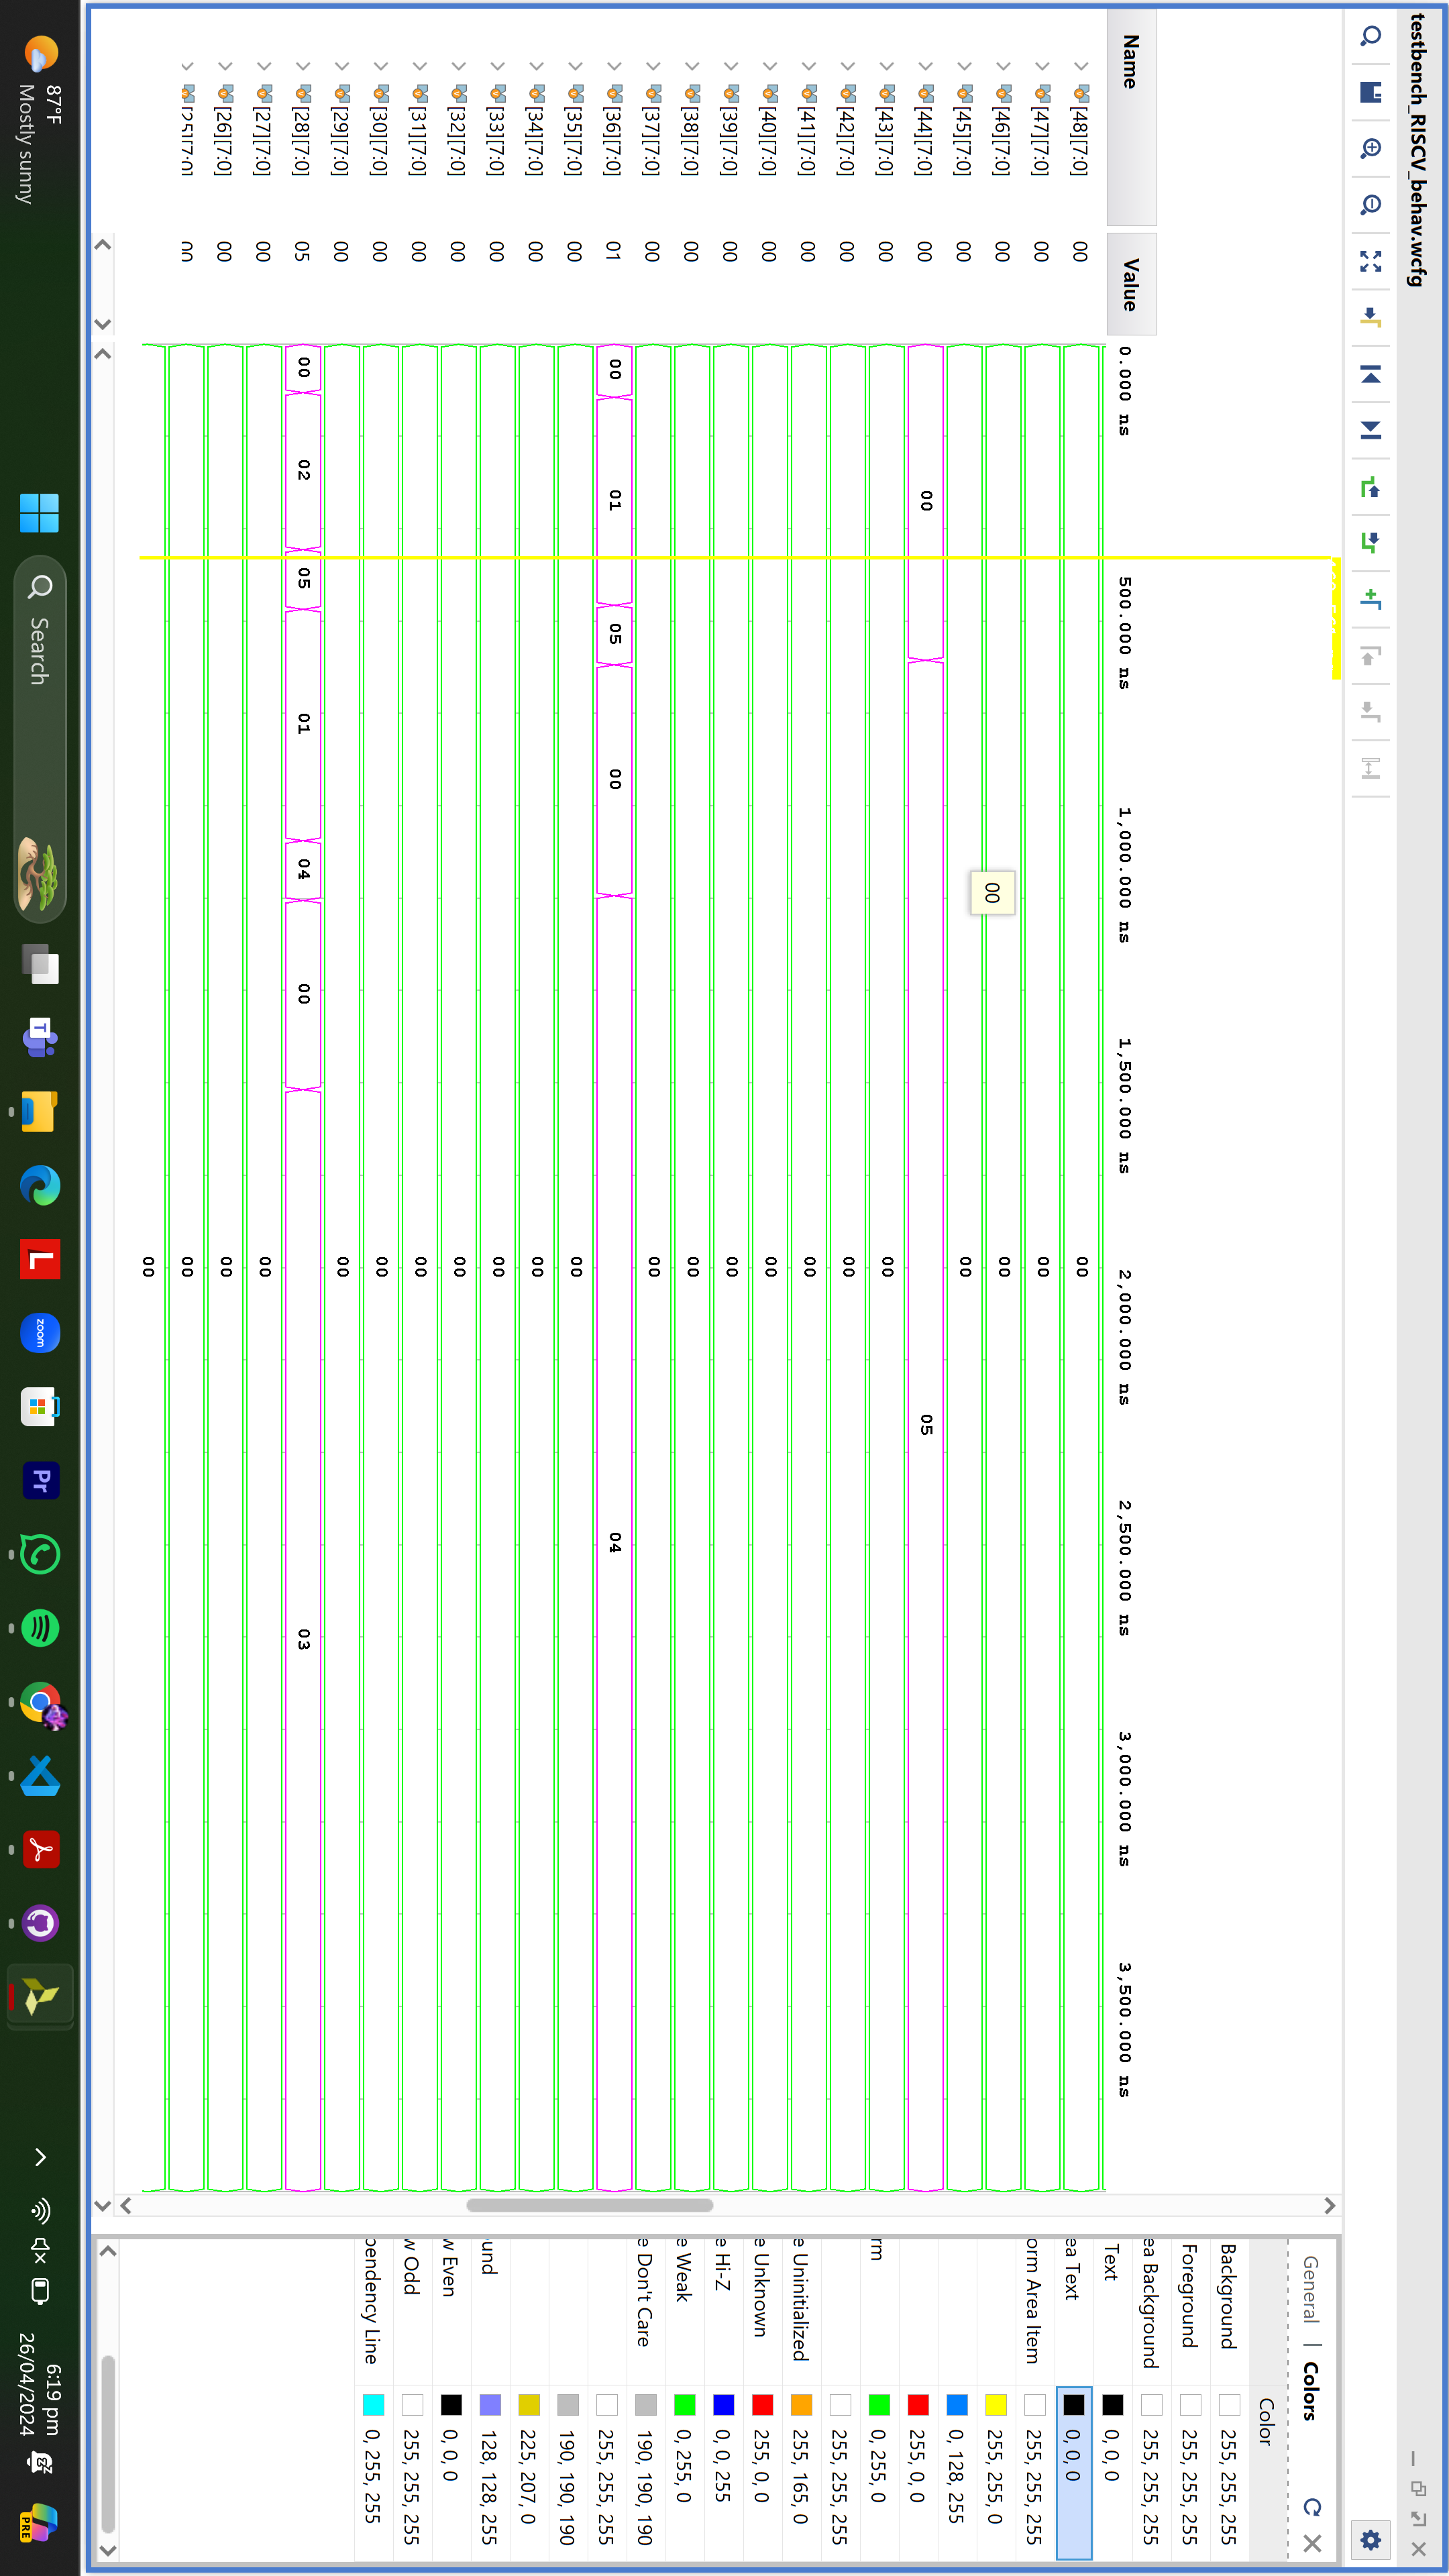
\includegraphics[scale = 0.5]{SingleCycle1.jpg}}
    \caption{Single Cycle Simulation 1}
\end{figure}

\begin{figure}[h]
    \centerline{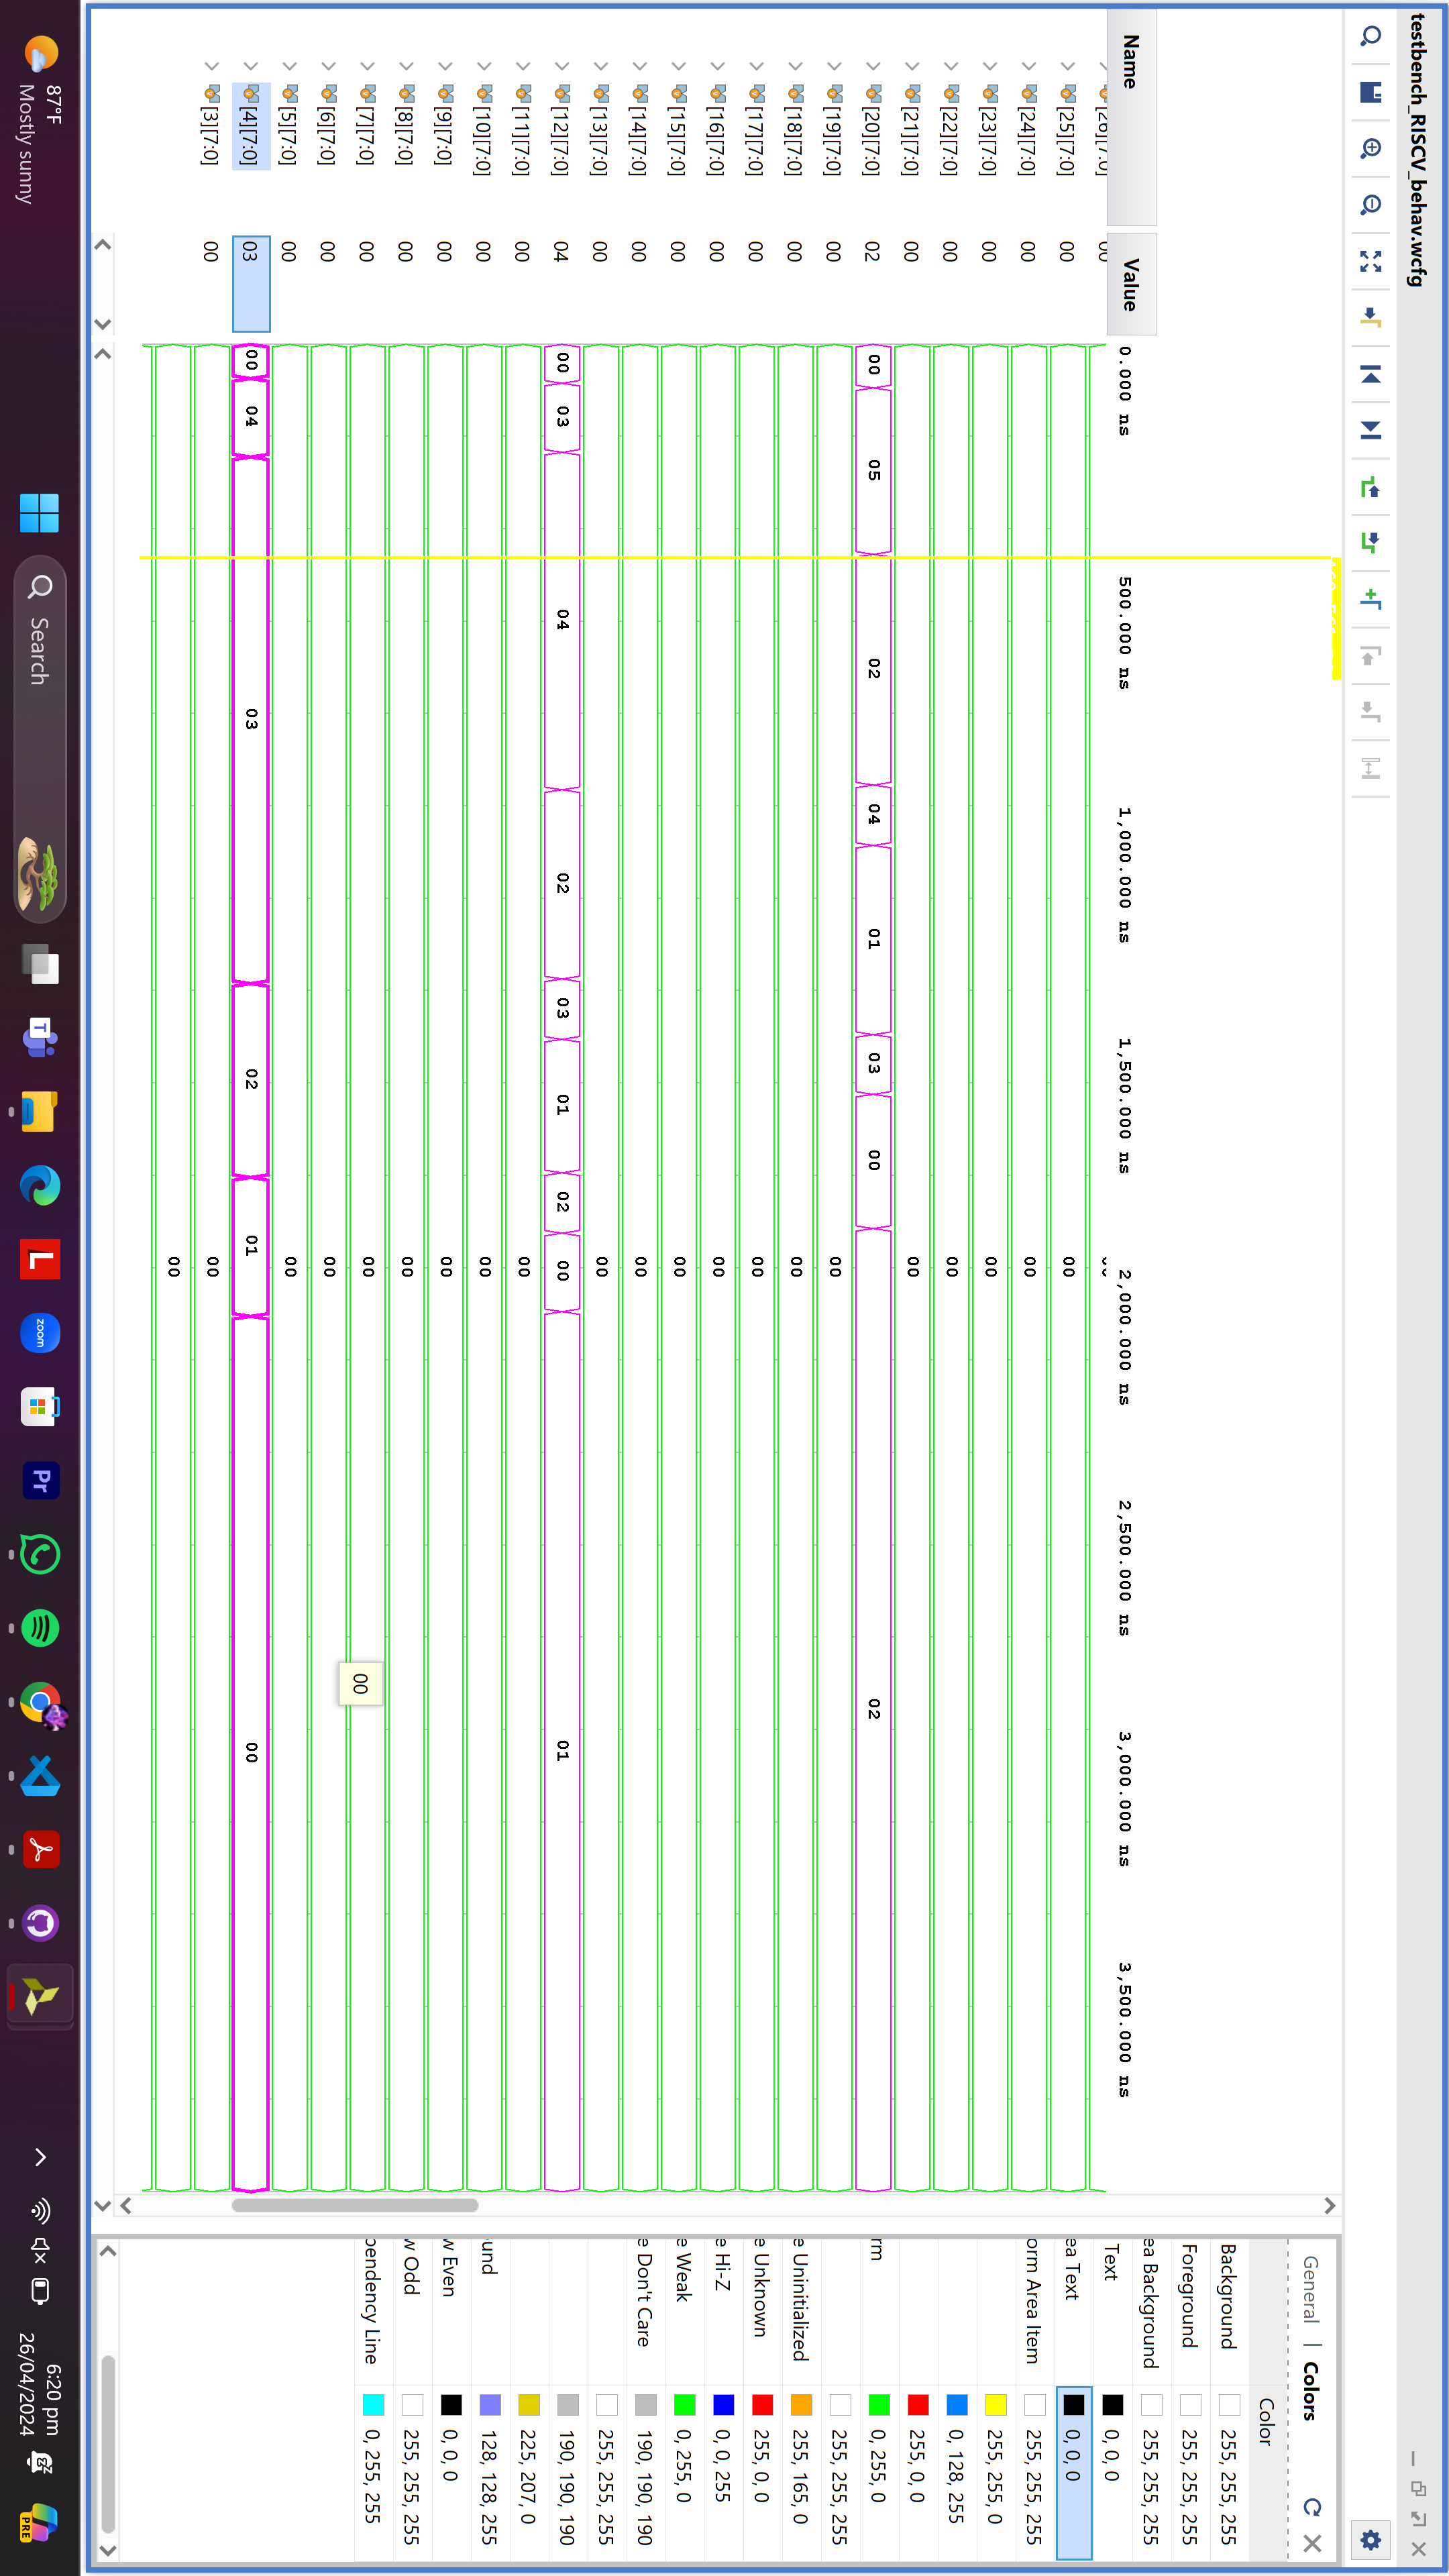
\includegraphics[scale = 0.5]{SingleCycle2.jpg}}
    \caption{Single Cycle Simulation 2}
\end{figure}

\newpage
\subsection{Synopsis}
    To make our sorting algorithm function properly, we introduced changes to the ALU and the final MUX module (by modifying the select line). Additionally, we added a new module called the Branch\_module.
\newpage
\section{Task2}
\subsection{Testing 5-Stage/Pipelined RISC V Processor for Sorting Algorithm}

Here we upgraded our previously developed processor for Pipeline Execution: Integration of 5 Stages and 4 New Modules.

\subsection{Changes}

To implement a pipelined design, the following modules were added to enable the staging to work effectively:
\begin{itemize}
\item IF\_ID
\item ID\_EX
\item EX\_MEM
\item MEM\_WB
\item Forwarding\_Unit
\end{itemize}

Each stage passes the data and instructions to the next stage through the 4 pipeline registers, which help to ensure the proper timing of the data flow and avoid data hazards. These stages and pipeline registers form the backbone of the pipelined processor's operation. The forwarding unit facilitates the forwarding of data between pipeline stages to resolve hazards and maintain proper data flow.

\subsection{Testing Forwarding Unit}

We upgraded our previously developed processor by implementing a Forwarding Unit, which involved adding the Forward Unit module. The forwarding path was then integrated with the pipeline register modules to ensure efficient data flow between stages of the pipeline. These modifications helped to resolve data hazards that may have arisen during the pipelined execution of instructions.
\pagebreak
\subsection{Code and Waveform}
The link for the code can be found \href{https://github.com/NehalNN10/CA-final-project/blob/5b606f284db6f33765f0c830730e5cee43c01f18/final_project/final_project.srcs/sources_1/new/pipelinedProcessor.v}{here}.

\begin{figure}[h]
    \centerline{\includegraphics[scale = 0.5]{PipelineCycle.jpg}}
    \caption{Pipelined Cycle Simulation}
\end{figure}

\section{Task 3}

\subsection{Handling Data Hazards}

To address hazards in our circuitry, we need to develop modules for detecting hazards and stalling the pipeline. The detection modules will identify where forwarding is required. Once detected, we can use the forward module to actually perform the forwarding. Additionally, by rearranging non-dependent code statements with stalls, we can optimize our algorithm to work in fewer cycles.

\subsection{Changes}

In computer architecture, hazards refer to conflicts that arise when attempting to execute instructions in a pipelined processor. These conflicts can occur due to dependencies between instructions, leading to stalls or incorrect results.

To address this issue, we added a Hazard Detection Unit module to our processor. This module detects hazards and controls the pipeline by sending signals to flush or stall the pipeline. By adding this module, we improved the processor's efficiency and prevented errors caused by hazards.


The Hazard Detection Unit uses the input RS1, RS2, RD and MemRead signal to detect hazards in the pipeline. If a hazard is detected, the module signals the pipeline to either flush or stall the pipeline to prevent incorrect results. With this addition, our processor is better equipped to handle hazards and operate more efficiently.



\subsection{Code and Waveform}
The link to the code can be found \href{https://github.com/NehalNN10/CA-final-project/blob/5b606f284db6f33765f0c830730e5cee43c01f18/final_project/final_project.srcs/sources_1/new/hazardProcessor.v}{here}.

\begin{figure}[h!]
    \centerline{\includegraphics[scale = 0.5]{Pipelined_RISCV.jpg}}
    \caption{Pipelined RISC-V Processor}

  \end{figure}
  
\subsection{Synopsis}

Although our 5-stage pipelined processor was functioning well, we encountered stalls in our code due to the requirement of the next value of a register in the subsequent line of code. This necessitates a sequential code and environment, causing the processor to pause for several cycles before resuming the sequence.

To address this issue, we incorporated flush and stall signals into our processor. These signals allow us to mitigate stalls and enable the processor to operate at a faster pace. With this improvement, our processor can continue functioning without delays caused by sequential code.

\chapter{Conclusion and Challenges}

Building the processor required significant brainpower, and we faced challenges with EDA crashing at critical moments, which taught us a great deal. According to theory, pipelined processors are faster than single-cycle processors because they don't wait for the entire instruction to execute. This makes them highly effective for parallel computing or asynchronous programming.

With better hazard handling, our processor can work even faster and more effectively. Although we faced stalls in our sorting algorithm due to time and complexity limitations, better hazard and stall units can mitigate these issues.

Implementing a real processor through gate-level logic has given us a deeper appreciation for Digital Logic Design.

\chapter{Comparison}

Pipelined processors are typically designed to be faster than non-pipelined processors, with a potential speedup of up to four times. However, in our case, the pipelined processor is not functioning optimally, with a latency of 3000ns, which is longer than the 1500ns latency of the non-pipelined processor. This suggests that there may be issues with pipeline hazards, control, or other design problems that are affecting the efficiency of your processor. To improve the performance of our pipelined processor, we need to analyze and optimize its design.

\chapter{Task Division}
\begin{itemize}
    \item {\large \underline{Nehal}: Bubble Sort Code and Single Cycle Processor}
    \item {\large \underline{Shawaiz and Aina}: Pipelined Processor and Debugging}
    \item {\large \underline{All Three}: Debugging and Integration}
\end{itemize}

\chapter{References}

[1] HU-LMS. Book. \textit{Course Book}. Computer Organization and Design: The Hardware/Software Interface RISC-V Edition by David A. Patterson, John L. Hennessy

\appendix
\chapter{Appendix}

GitHub links for codes of different processors: 
\begin{itemize}
    \item Single Cycle Processor (Task 1): \url{https://github.com/NehalNN10/CA-final-project/blob/5b606f284db6f33765f0c830730e5cee43c01f18/final_project/final_project.srcs/sources_1/new/RISCV_Processor.v}
    \item Pipelined Processor (Task 2): \url{https://github.com/NehalNN10/CA-final-project/blob/5b606f284db6f33765f0c830730e5cee43c01f18/final_project/final_project.srcs/sources_1/new/pipelinedProcessor.v}
    \item Pipelined Processor with Hazard Detection (Task 3): \url{https://github.com/NehalNN10/CA-final-project/blob/5b606f284db6f33765f0c830730e5cee43c01f18/final_project/final_project.srcs/sources_1/new/hazardProcessor.v}
\end{itemize}

\end{document}